\chapter{Resultados}\label{cap:resultados}

% \MexerDepois{Escrever algo aqui}

Neste capítulo, são apresentados detalhes sobre a construção do banco de imagens utilizado ao longo do desenvolvimento do trabalho, bem como são levantados detalhes sobre a performance geral atingida e comparando com a performance de uma versão simplificada do sistema.
Também são apontandos problemas encontrados ao longo do desenvolvimento do trabalho.

\section{Construção do banco de imagens}

O banco de imagens foi criado utilizando fotos de embalagens de medicamentos, contendo ampolas, bisnagas, caixas, cartelas, frascos, sachês, entre outros.
Grande parte das fotos foi tirada visando contornar os problemas encontrados, citados na \autoref{sec:problemas}.

Parte dos medicamentos registrados não constam no sistema do Bulário Eletrônico da \ac{Anvisa}, como suplementos alimentares ou medicamento veterinários.
Nota-se também que as imagens apresentam diferentes resoluções, estas foram dividias em três grupos:
\begin{itemize}
    \item Baixa resolução, abaixo de \SI{0.92}{\mega\pixel} (HD) \cite{makiyama2022Imagens};
    \item Média resolução, entre \SI{0.92}{\mega\pixel} (HD) e \SI{3.69}{\mega\pixel} (QHD) \cite{makiyama2022Imagens};
    \item Alta resolução, acima de \SI{3.69}{\mega\pixel} (QHD) \cite{makiyama2022Imagens}.
\end{itemize}
A \autoref{tab:banco} sumariza informações sobre características do banco contruído.

\begin{table}[htbp]
    \centering
    \caption{Informações sobre o banco de fotos criado, contando quantidade de imagens, se estão presentes ou ausentes no Bulário Eletrônico da \ac{Anvisa} e resolução.}
    \pgfplotstabletypesetfile{../data/banco.dat}
    \medskip
    \caption*{Fonte: Autor.}
    \label{tab:banco}
\end{table}

% \MexerDepois{Detalhar banco de imagens}

\section{Performance}

A análise de performance trata-se relação entre acertos ou falhas com a quantidade total de testes realizados pelo sistema.

\subsection{Caso geral de leitura de texto}

O caso geral aborda a lista completa de imagens do banco construído, verificando quais dessas tiveram seu texto lido corretamente e quais medicamentos foram localizados com sucesso no sistema do Bulário Eletrônico da \ac{Anvisa}.
A \autoref{tab:geral} apresenta a relação de acurácias para sucesso de leitura e para sucesso de busca pelo nome localizado.
É importante notar que na primeira linha da tabela, casos de leituras incorretas, não existem casos de remédios encontrados no Bulário Eletrônico, já que não haveriam termos para encontrá-los.

\begin{table}[htbp]
    \centering
    \caption{Acurácia geral do sistema, destaque para casos lidos parcial ou corretamente.}
    \pgfplotstabletypesetfile{../data/geral.dat}
    \medskip
    \caption*{Fonte: Autor.}
    \label{tab:geral}
\end{table}

\subsection{Caso de busca de termos}

O caso de busca de termos aborda somente a lista de imagens que tiveram seu texto lido corretamente, verificando quais medicamentos foram localizados com sucesso.
Essa análise tem relação com a ordem que os termos localizados são buscados no Bulário Eletrônico do \ac{Anvisa}.
A \autoref{tab:lido} apresenta a relação de acurácias para sucesso de leitura e para sucesso na busca pelo nome localizado.
É válido notar que são consideradas leituras totalmente corretas e parcialmente corretas do nome do medicamento na imagem.

\begin{table}[htbp]
    \centering
    \caption{Acurácia do sistema somente para casos lidos corretamente, destaque para casos localizados corretamente ou semelhantes.}
    \pgfplotstabletypesetfile{../data/lido.dat}
    \medskip
    \caption*{Fonte: Autor.}
    \label{tab:lido}
\end{table}

\subsection{Comparação com busca sem versões alternativas}

Também foi realizada uma análise alternativa dos métodos adotados, porém neste caso, somente utilizando a imagem em sua versão original, sem separação de componentes de cores ou diferentes codificações.
Neste caso, conforme apresentado na \autoref{tab:geral_raw}, a maioria das imagens apresentou falha na leitura, sem conseguir encontrar termos que pudessem levar à localização do medicamento no sistema do Bulário Eletrônico da \ac{Anvisa}.

\begin{table}[htbp]
    \centering
    \caption{Acurácia geral do sistema sem versões alternativas de imagem.}
    \pgfplotstabletypesetfile{../data/geral_raw.dat}
    \medskip
    \caption*{Fonte: Autor.}
    \label{tab:geral_raw}
\end{table}

Novamente denotando somente os resultados onde a busca textual foi realizada corretamente, a \autoref{tab:lido_raw} traz a relação de corretude das buscas realizadas nestes termos.
Apesar dos números parecerem promissores, é importante ressaltar que são referentes a menos de \SI{30}{\percent} das fotos que compõe o banco de dados.

\begin{table}[htbp]
    \centering
    \caption{Acurácia do sistema sem versões alternativas de imagem somente para casos lidos corretamente.}
    \pgfplotstabletypesetfile{../data/lido_raw.dat}
    \medskip
    \caption*{Fonte: Autor.}
    \label{tab:lido_raw}
\end{table}


\section{Problemas Encontrados}\label{sec:problemas}

Ao longo do desenvolvimento e testes do sistema, alguns problemas foram encontrados, essa seção os denota, pontuando os detalhes, suas causas e implicações gerais na performance.

\subsection{Falhas de acesso}

Notou-se que o site do Bulário Eletrônico pode ficar \textit{offline} ou apresentar problemas de conexão fora do período comercial, \ie\ fora do período de \SI{8}{\hour} às \SI{18}{\hour}, de Segunda à Sexta.
Nesse caso, o sistema desenvolvido não conseguirá realizar busca por qualquer medicamento, mesmo que tenha encontrado o nome correto na imagem, a \autoref{fig:fail:domingo} apresenta um exemplo deste caso.

As Figuras \ref{fig:fail:404} e \ref{fig:fail:timeout} apresentam registros de falhas de acesso ao site de consultas ao Bulário Eletrônico, ambos os casos ocorreram fora do horário comercial.

\begin{figure}[htbp]
    \centering
    \caption{Sistema tentando acessar o Bulário Eletrônico, fora do horário comercial.}
    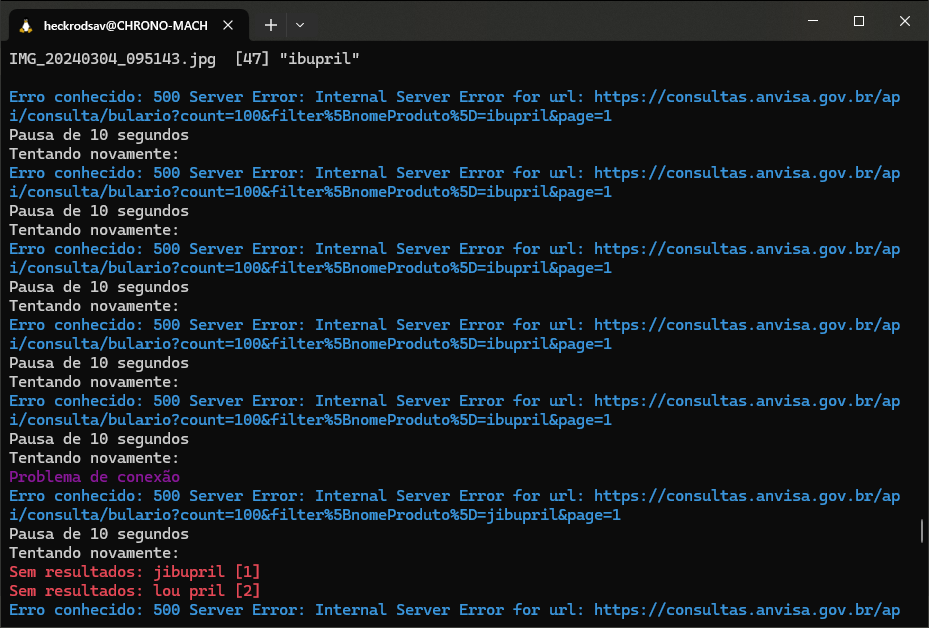
\includegraphics[width=0.95\linewidth]{../pictures/Anvisa_domingo.png}
    \caption*{Fonte: Autor, captura realizada em 2024-03-13.}
    \label{fig:fail:domingo}
\end{figure}

\begin{figure}[htbp]
    \centering
    \caption{Bulário Eletrônico com erro 404, fora do horário comercial.}
    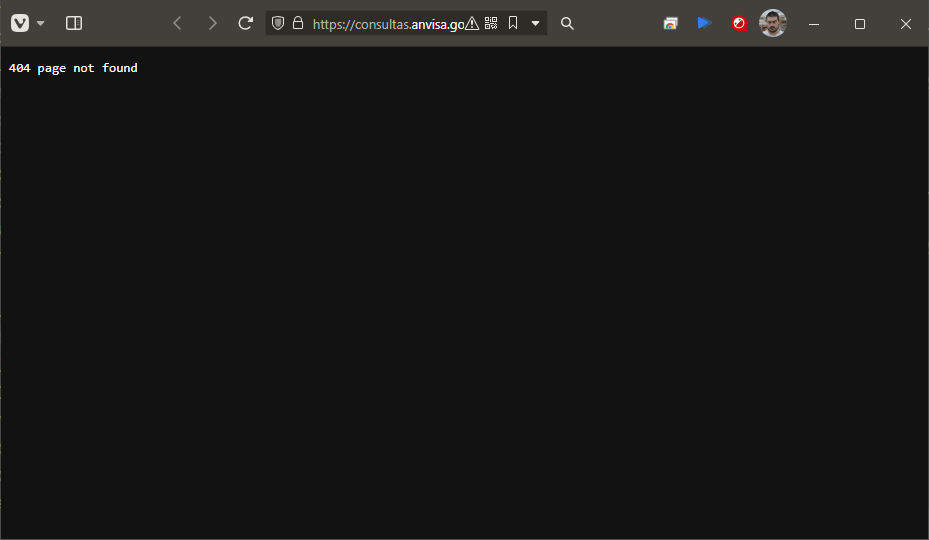
\includegraphics[width=0.95\linewidth]{../pictures/Anvisa_error_404.png}
    \caption*{Fonte: Autor, captura realizada em 2024-03-13.}
    \label{fig:fail:404}
\end{figure}

\begin{figure}[htbp]
    \centering
    \caption{Erro no servidor do Bulário Eletrônico, fora do horário comercial.}
    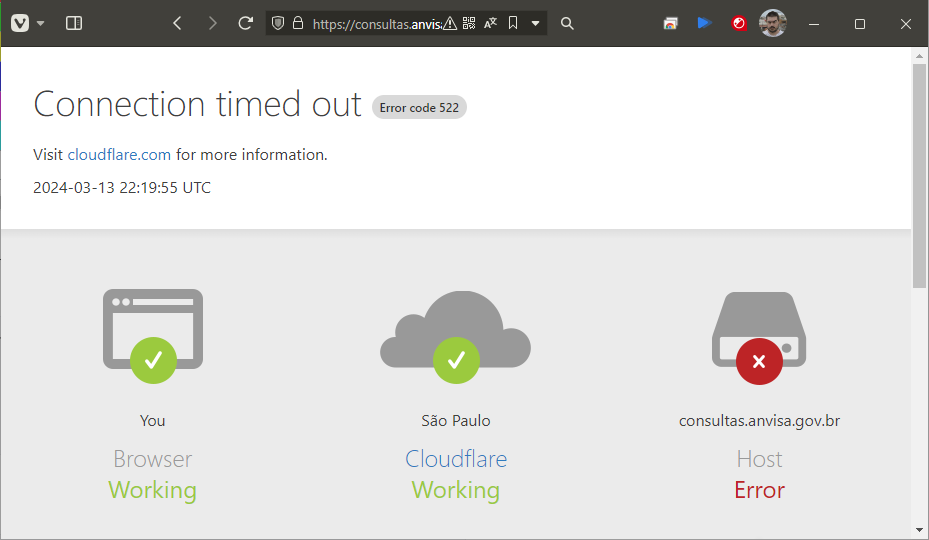
\includegraphics[width=0.95\linewidth]{../pictures/Anvisa_error_timeout.png}
    \caption*{Fonte: Autor, captura realizada em 2024-03-13.}
    \label{fig:fail:timeout}
\end{figure}

\subsection{Orientação do texto}

Outro problema notado é referente à orientação do texto nas imagens utilizadas.
Quando o texto não está paralelo à horizontal da imagem, o motor \ac{OCR} utilizado falha em realizar a identificação.
Neste contexto, o banco de imagens foi construído para contornar este problema.
As Figuras \ref{fig:fotos:diagonal} e \ref{fig:fotos:horizontal} apresentam exemplos de falha e sucesso, respectivamente, para uma mesma embalagem de medicamento, a diferença nos dois casos é a orientação do texto.


\begin{figure}[htbp]
    \centering
    \caption{Fotos de medicamento com diferentes orientações de texto: diagonal (\subref{fig:fotos:diagonal}) e paralela (\subref{fig:fotos:horizontal}) à horizontal.}
    \hfill
    \begin{subfigure}[t]{0.45\textwidth}
        \centering
        \caption{Orientação diagonal à horizontal.}
        \label{fig:fotos:diagonal}
        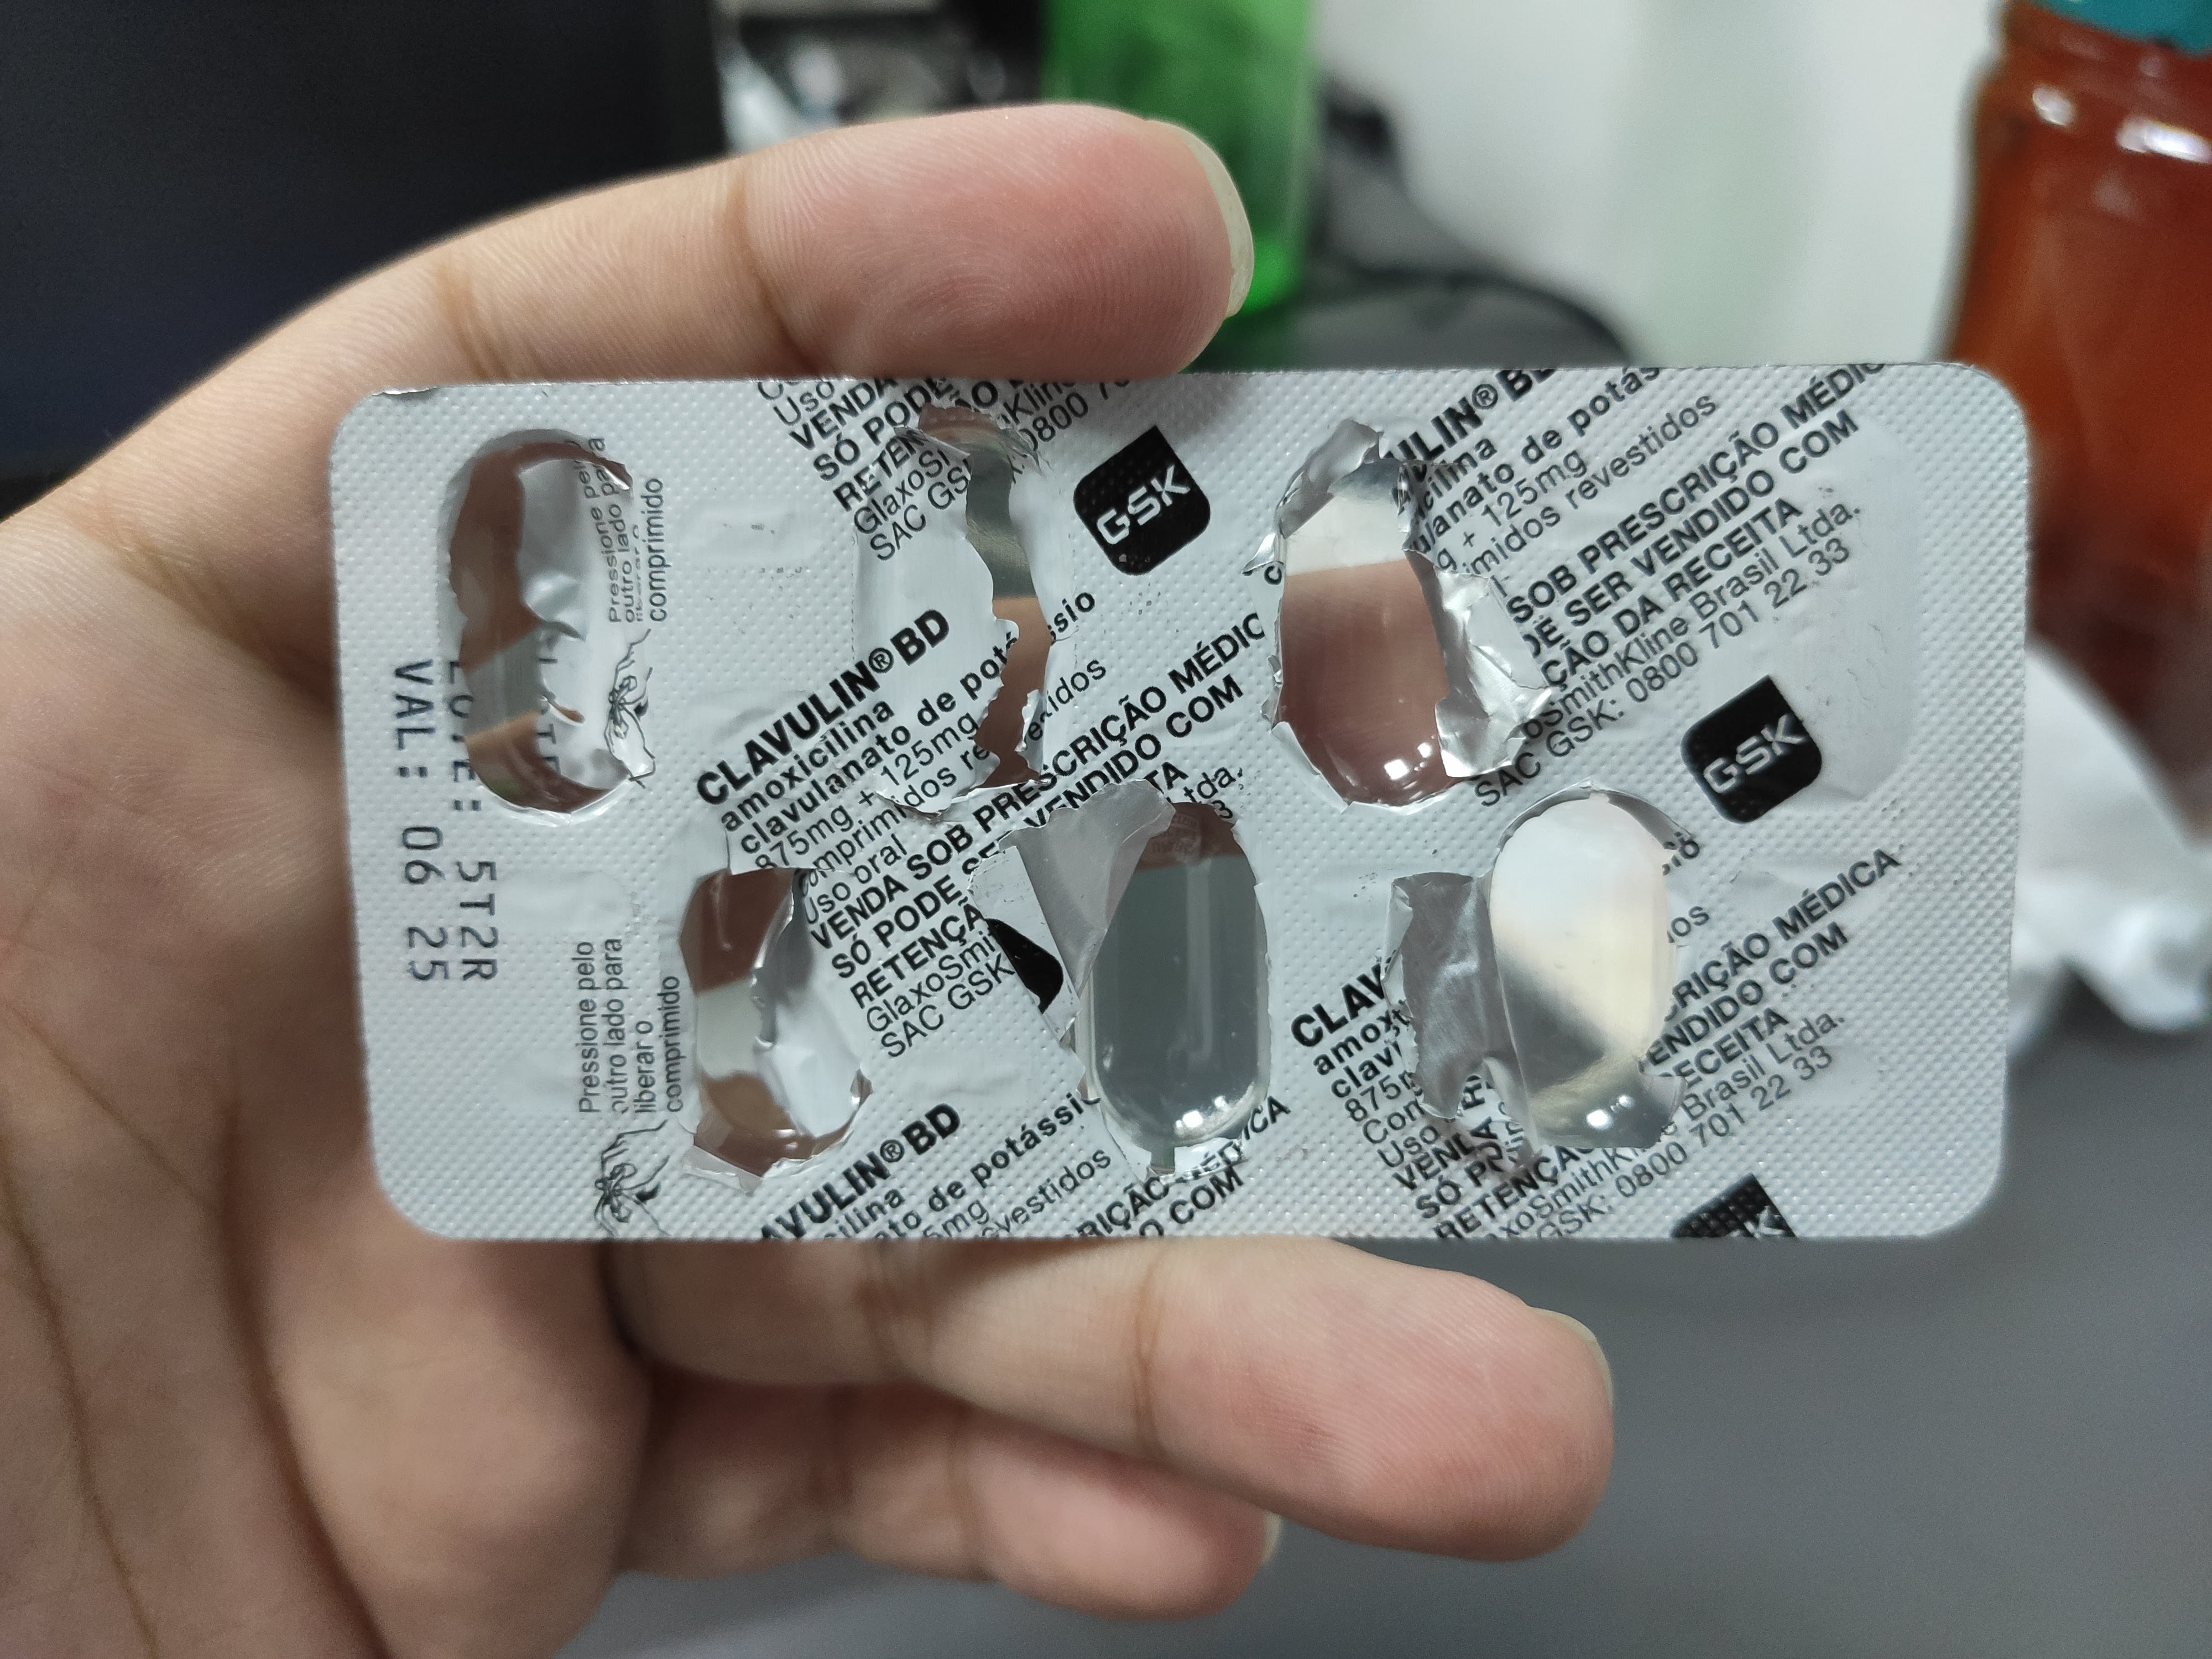
\includegraphics[width=\linewidth]{../pictures/IMG_20240229_162005.jpg}
        \caption*{Fonte: Autor.}
    \end{subfigure}
    \hfill
    \begin{subfigure}[t]{0.45\textwidth}
        \centering
        \caption{Orientação paralela à horizontal.}
        \label{fig:fotos:horizontal}
        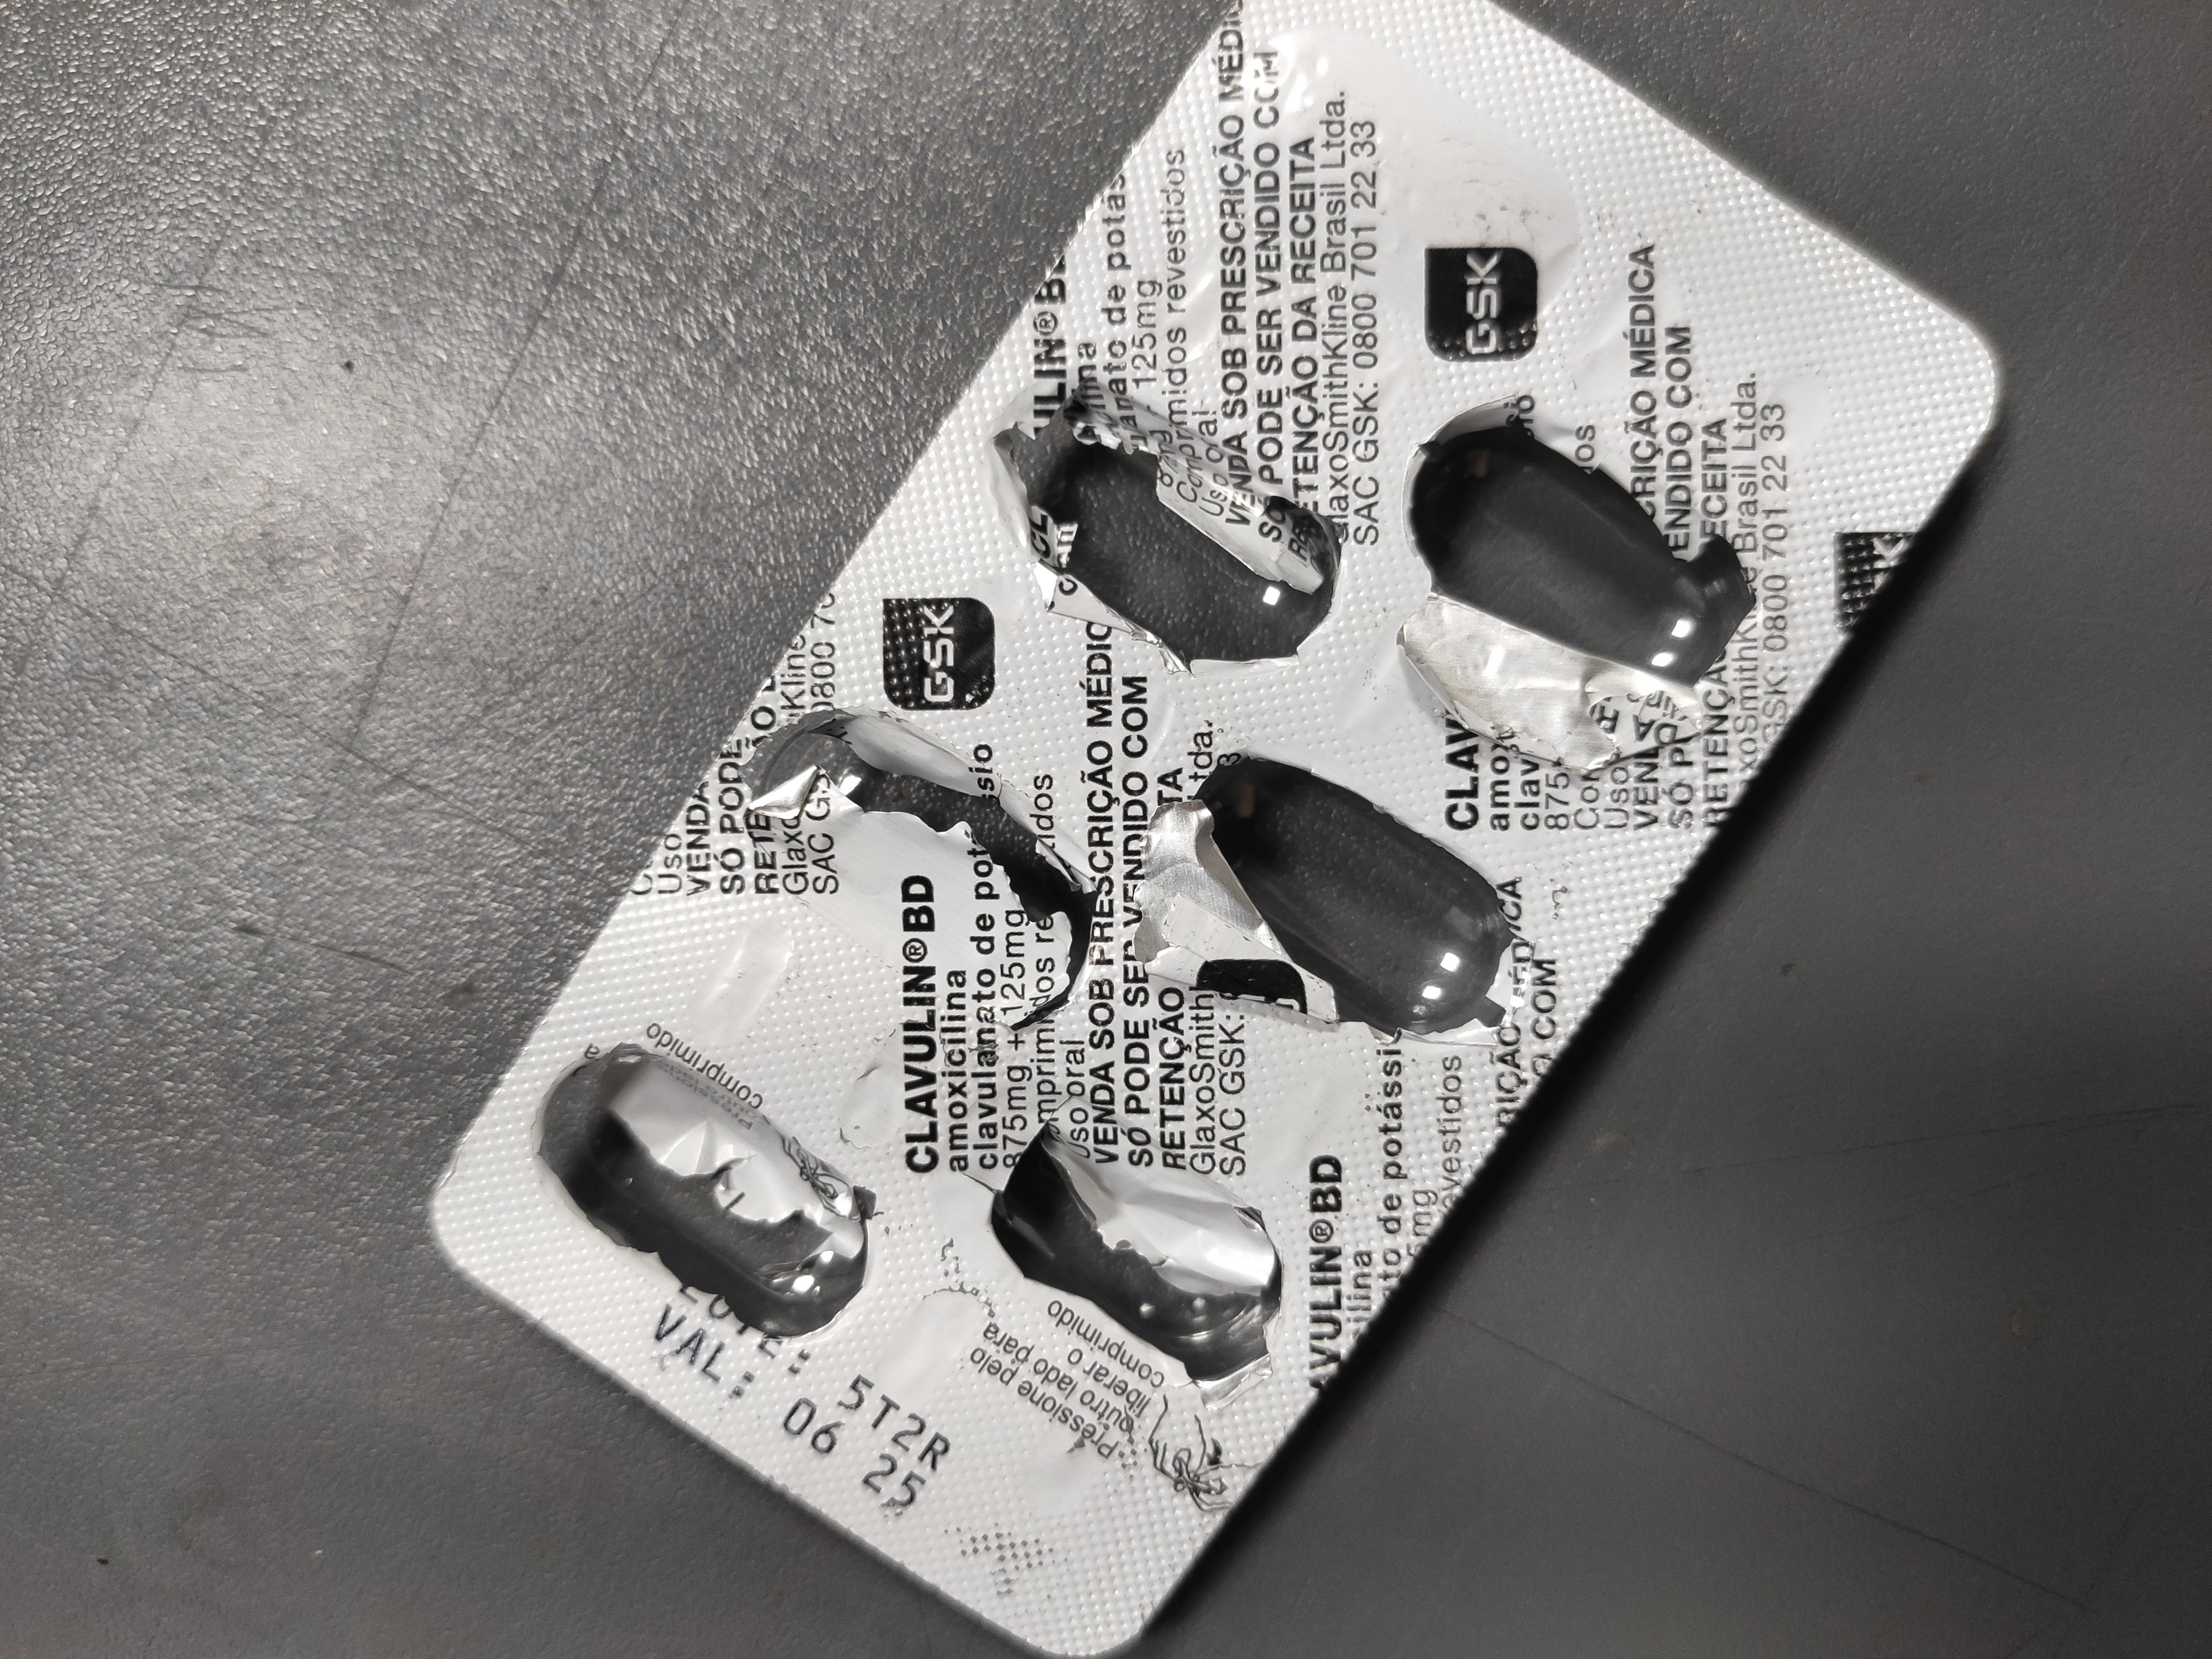
\includegraphics[width=\linewidth, angle=-90]{../pictures/IMG_20240307_185809.jpg}
        \caption*{Fonte: Autor.}
    \end{subfigure}
    \hfill
    \label{fig:fotos:diagvert}
\end{figure}

\subsection{Reflexos na imagem}

Também foi notado problemas relacionados a reflexos na região do texto de interesse das fotos.
Nestes casos, nenhuma das versões de diferentes codificações de cores foram capazes de interpretar corretamente o texto.
O sistema construído não conta com recursos para tentar completar as letras faltantes nesse contexto, então não consegue localizar o medicamento no Bulário Eletrônico.

Nestes casos, se faz necessária a aquisição de uma nova foto.
As Figuras \ref{fig:fotos:reflexo} e \ref{fig:fotos:visivel} apresentam, respectivamente, exemplos de foto com e sem reflexos na região de interesse.

\begin{figure}[htbp]
    \centering
    \caption{Fotos de medicamento com (\subref{fig:fotos:reflexo}) e sem (\subref{fig:fotos:visivel}) reflexo na região do texto.}
    \hfill
    \begin{subfigure}[t]{0.45\textwidth}
        \centering
        \caption{Reflexo sobre texto de interesse.}
        \label{fig:fotos:reflexo}
        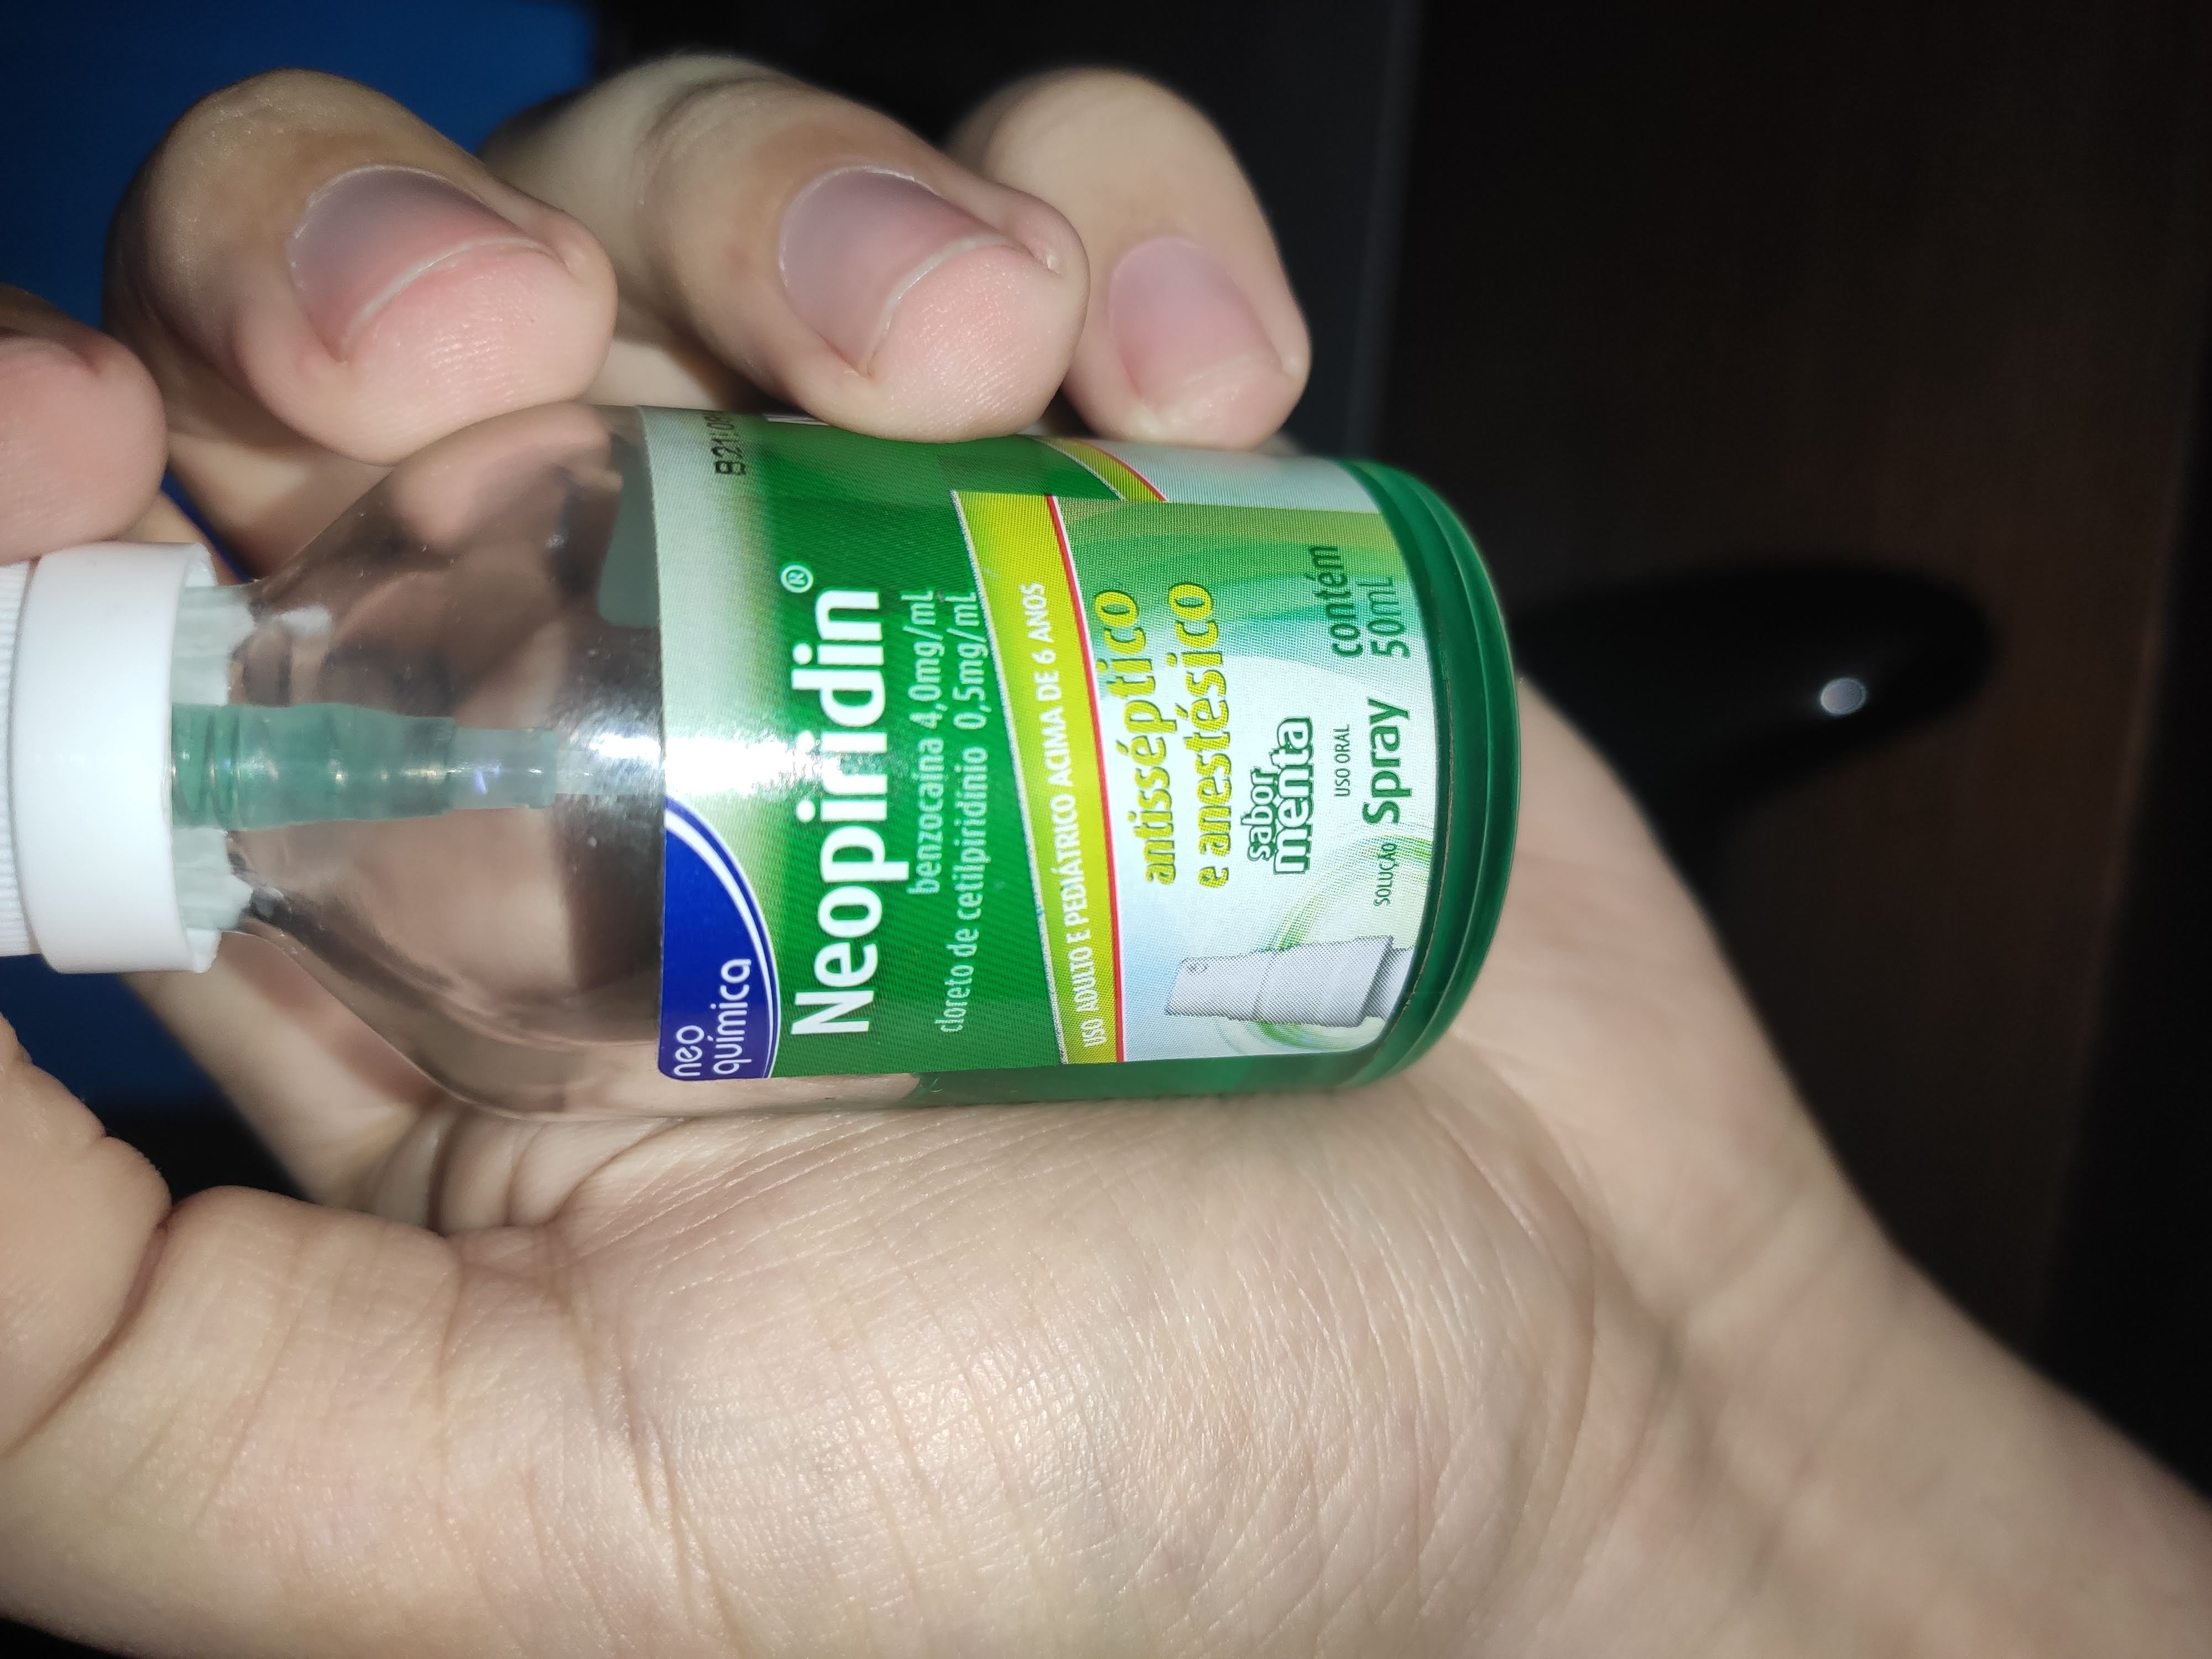
\includegraphics[keepaspectratio, width=\linewidth, angle=-90]{../pictures/IMG_20220908_191849.jpg}
        \caption*{Fonte: Autor.}
    \end{subfigure}
    \hfill
    \begin{subfigure}[t]{0.45\textwidth}
        \centering
        \caption{Texto de interesse sem reflexo.}
        \label{fig:fotos:visivel}
        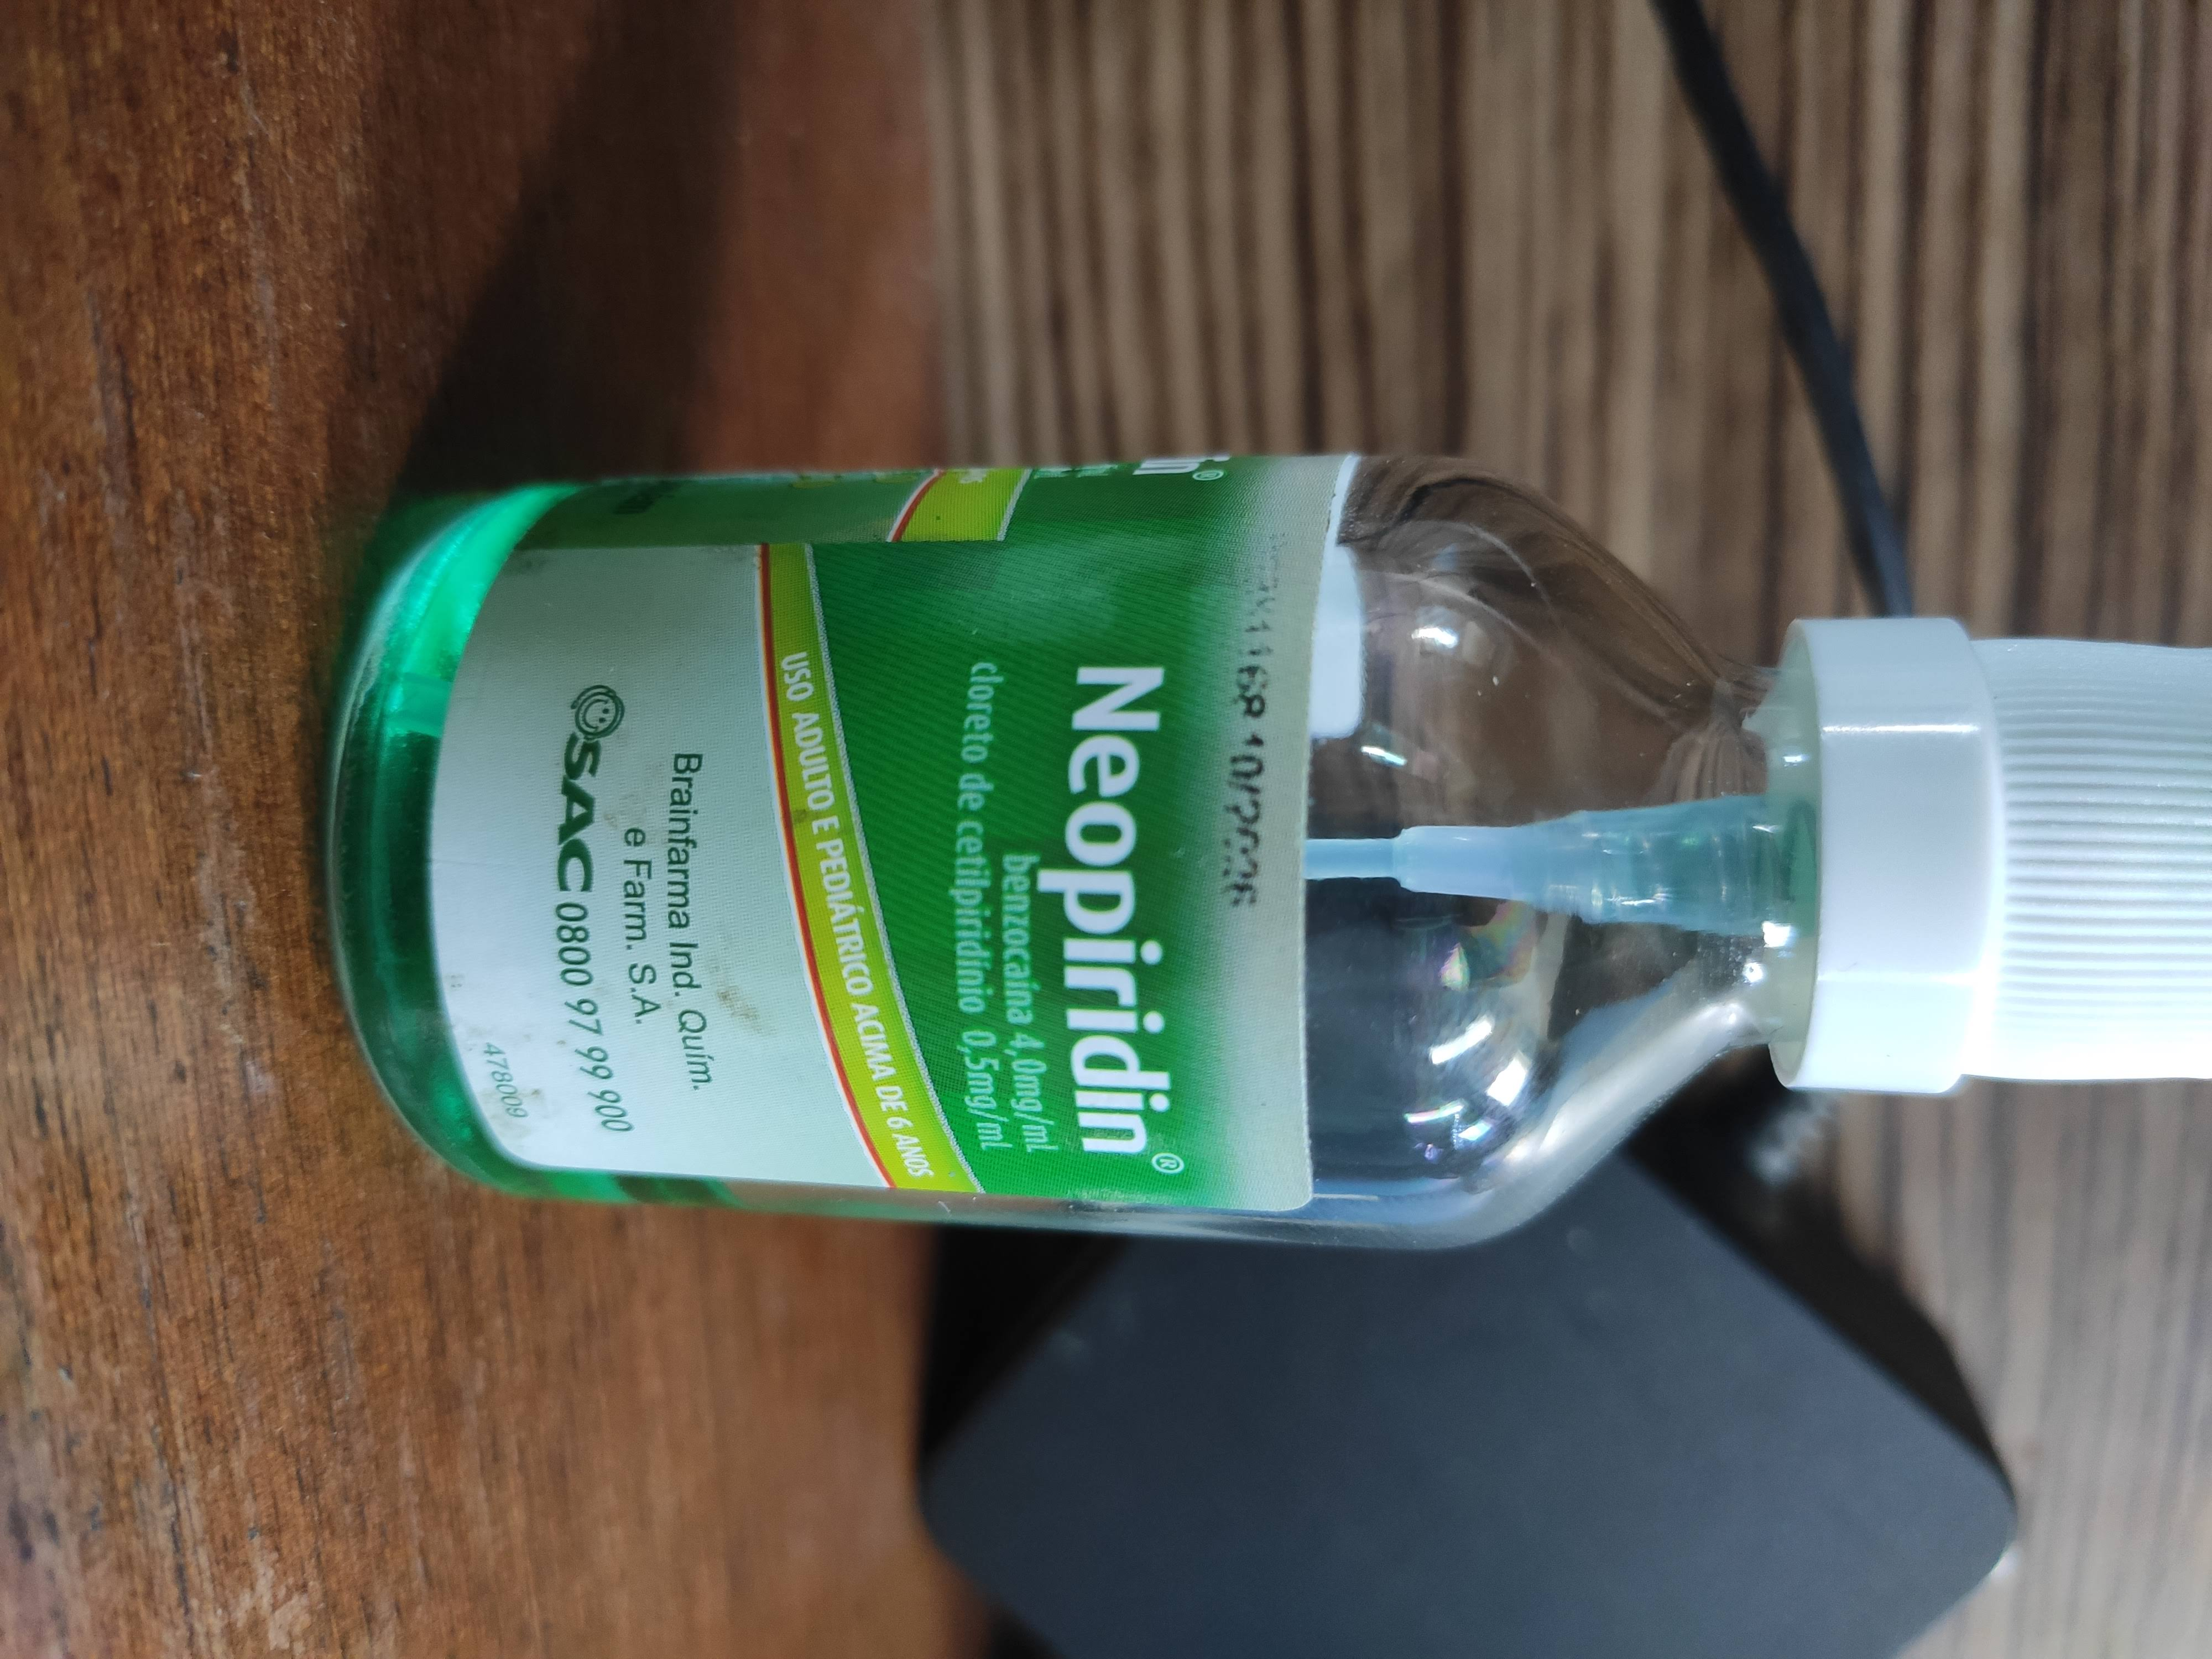
\includegraphics[keepaspectratio, width=\linewidth, angle=90]{../pictures/IMG_20240301_105852.jpg}
        \caption*{Fonte: Autor.}
    \end{subfigure}
    \hfill
    \label{fig:fotos:refvis}
\end{figure}

\subsection{Obstruções na embalagem}

Semelhante ao caso anterior, foi notado um problema quando a embalagem do medicamento apresenta alguma obstrução, como adesivos, carimbos e principalmente cortes na região do texto.
Geralmente encontrado em fotos de cartelas de comprimidos, essas obstruções podem alterar a visibilidade de alguma parte do texto de interesse, impedindo a leitura.
As Figuras \ref{fig:fotos:quebrado} e \ref{fig:fotos:inteiro} apresentam, respectivamente, exemplos de foto com e sem obstrução na região de interesse.

\begin{figure}[htbp]
    \centering
    \caption{Fotos de medicamento com (\subref{fig:fotos:quebrado}) e sem (\subref{fig:fotos:inteiro}) rasuras na região do texto.}
    \hfill
    \begin{subfigure}[t]{0.45\textwidth}
        \centering
        \caption{Embalagem partida no texto.}
        \label{fig:fotos:quebrado}
        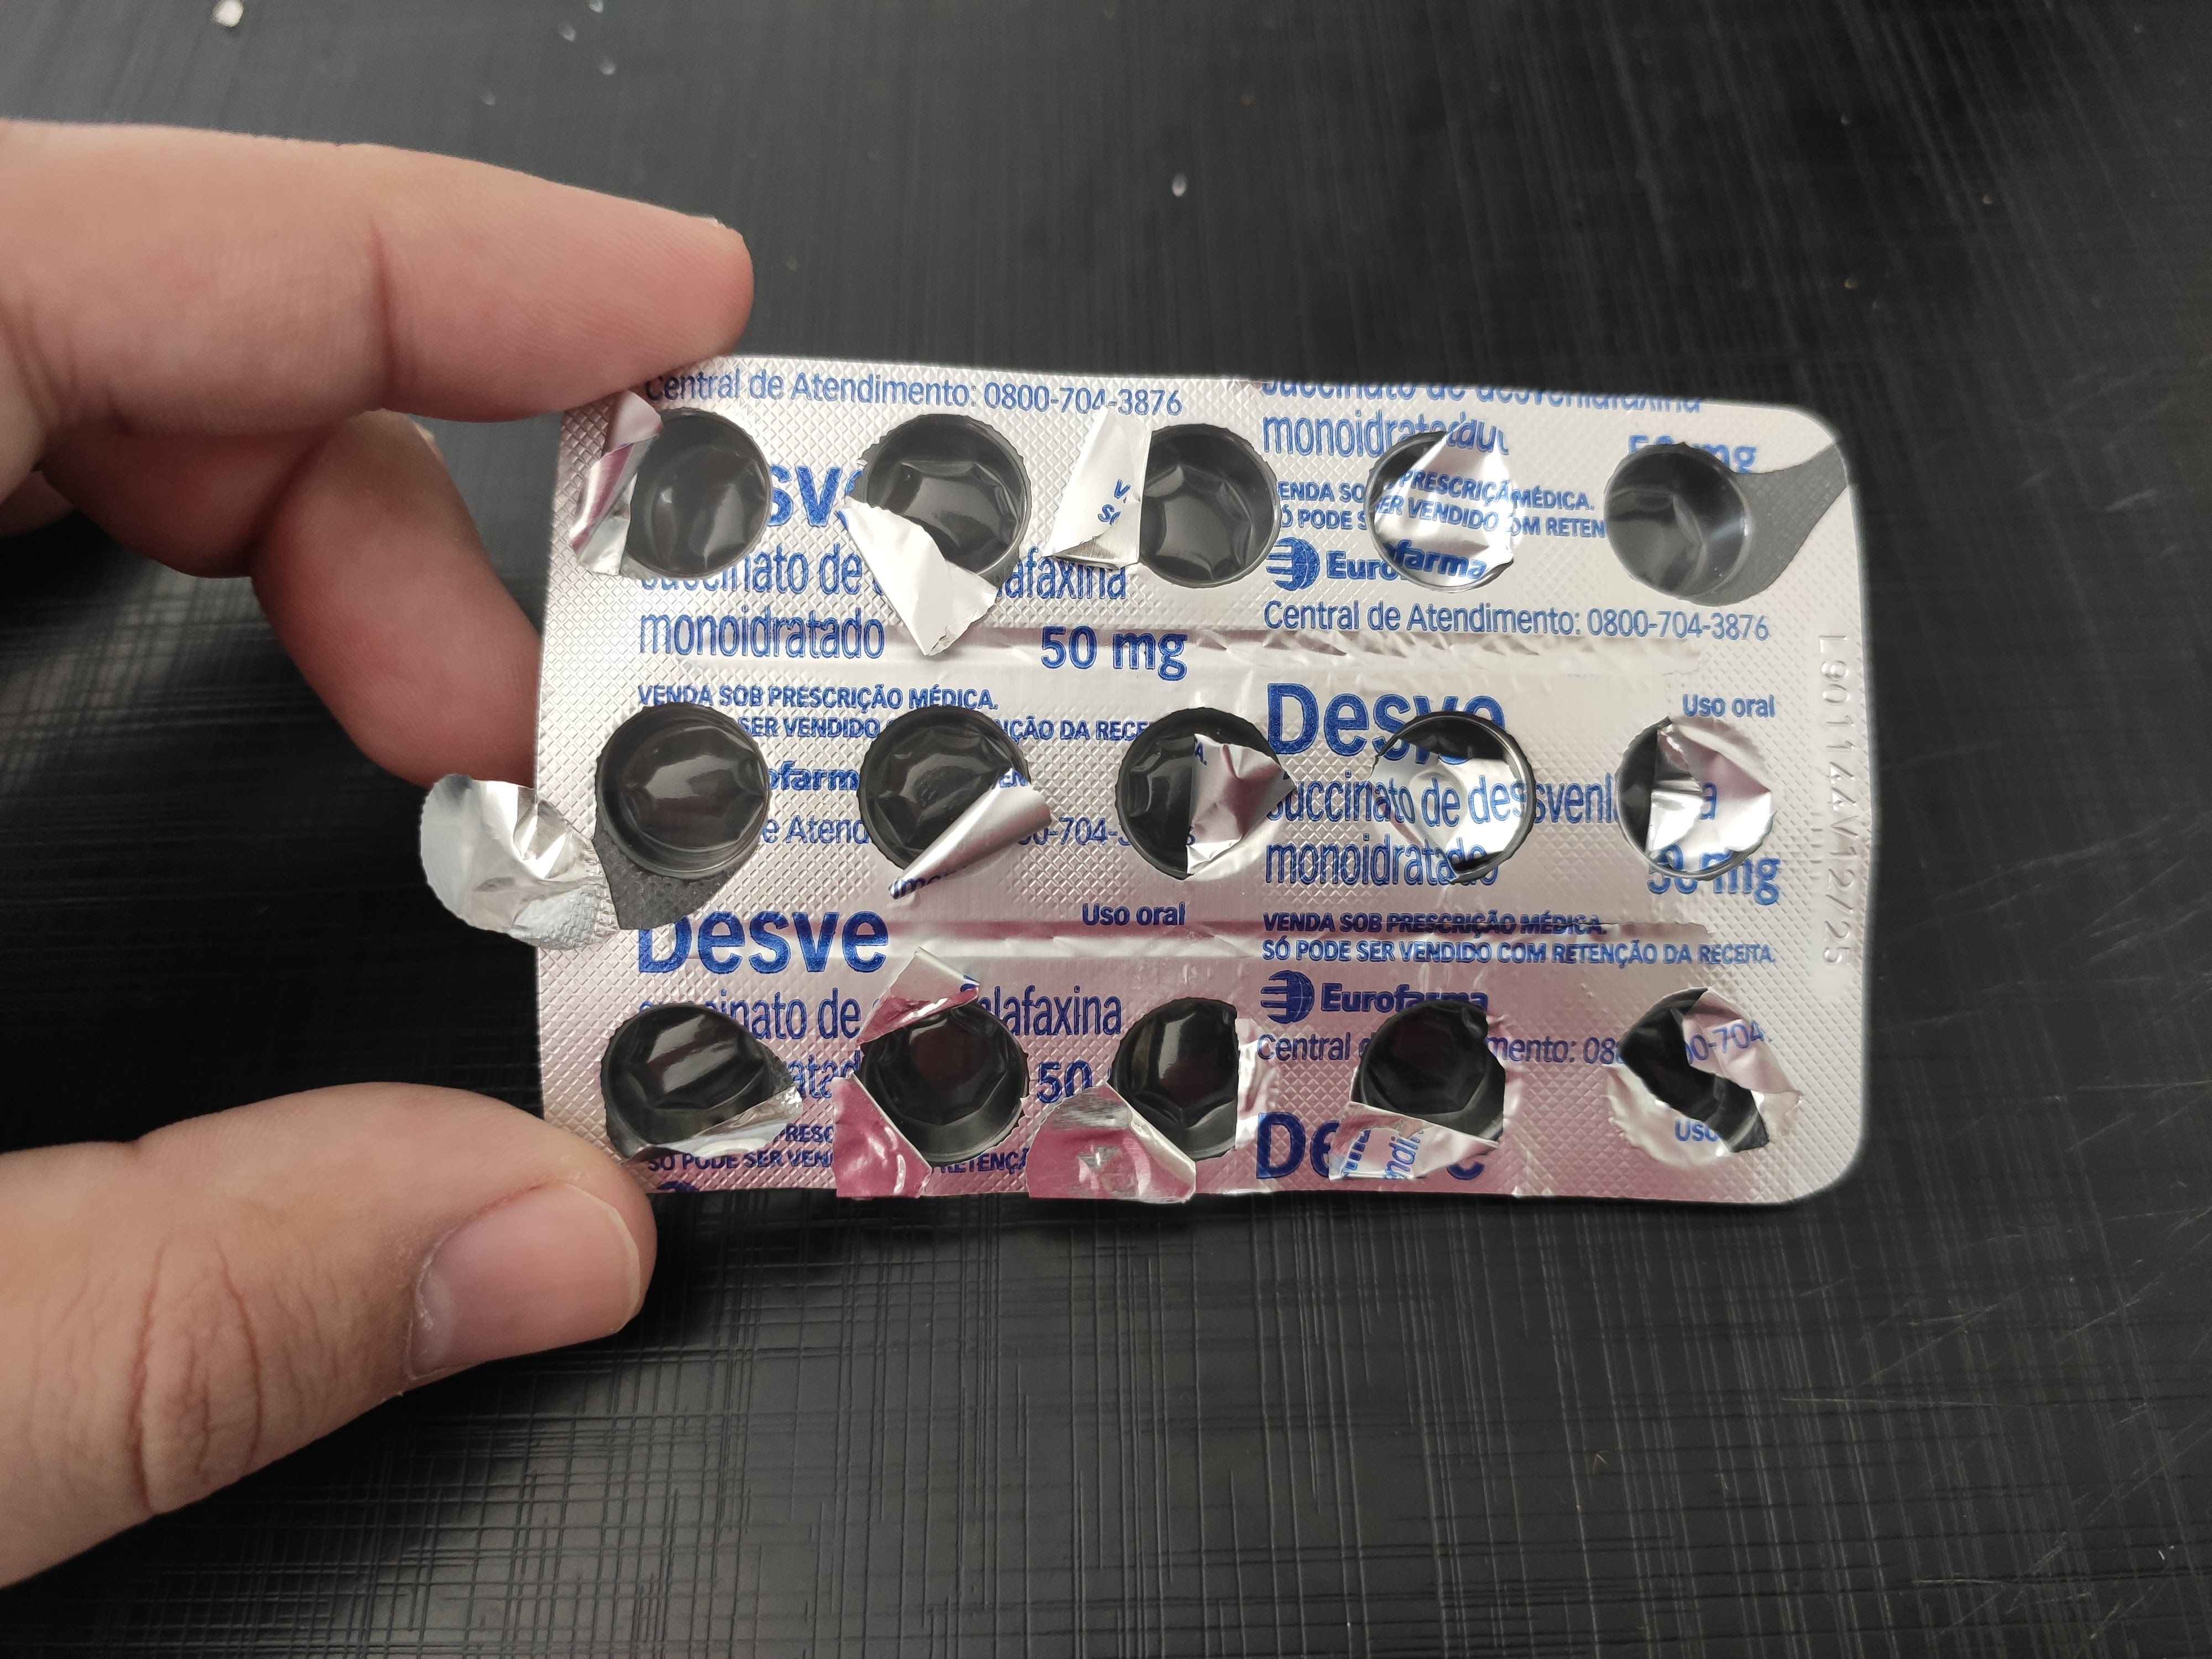
\includegraphics[width=\linewidth]{../pictures/IMG_20240725_110209.jpg}
        \caption*{Fonte: Autor.}
    \end{subfigure}
    \hfill
    \begin{subfigure}[t]{0.45\textwidth}
        \centering
        \caption{Embalagem com texto inteiro.}
        \label{fig:fotos:inteiro}
        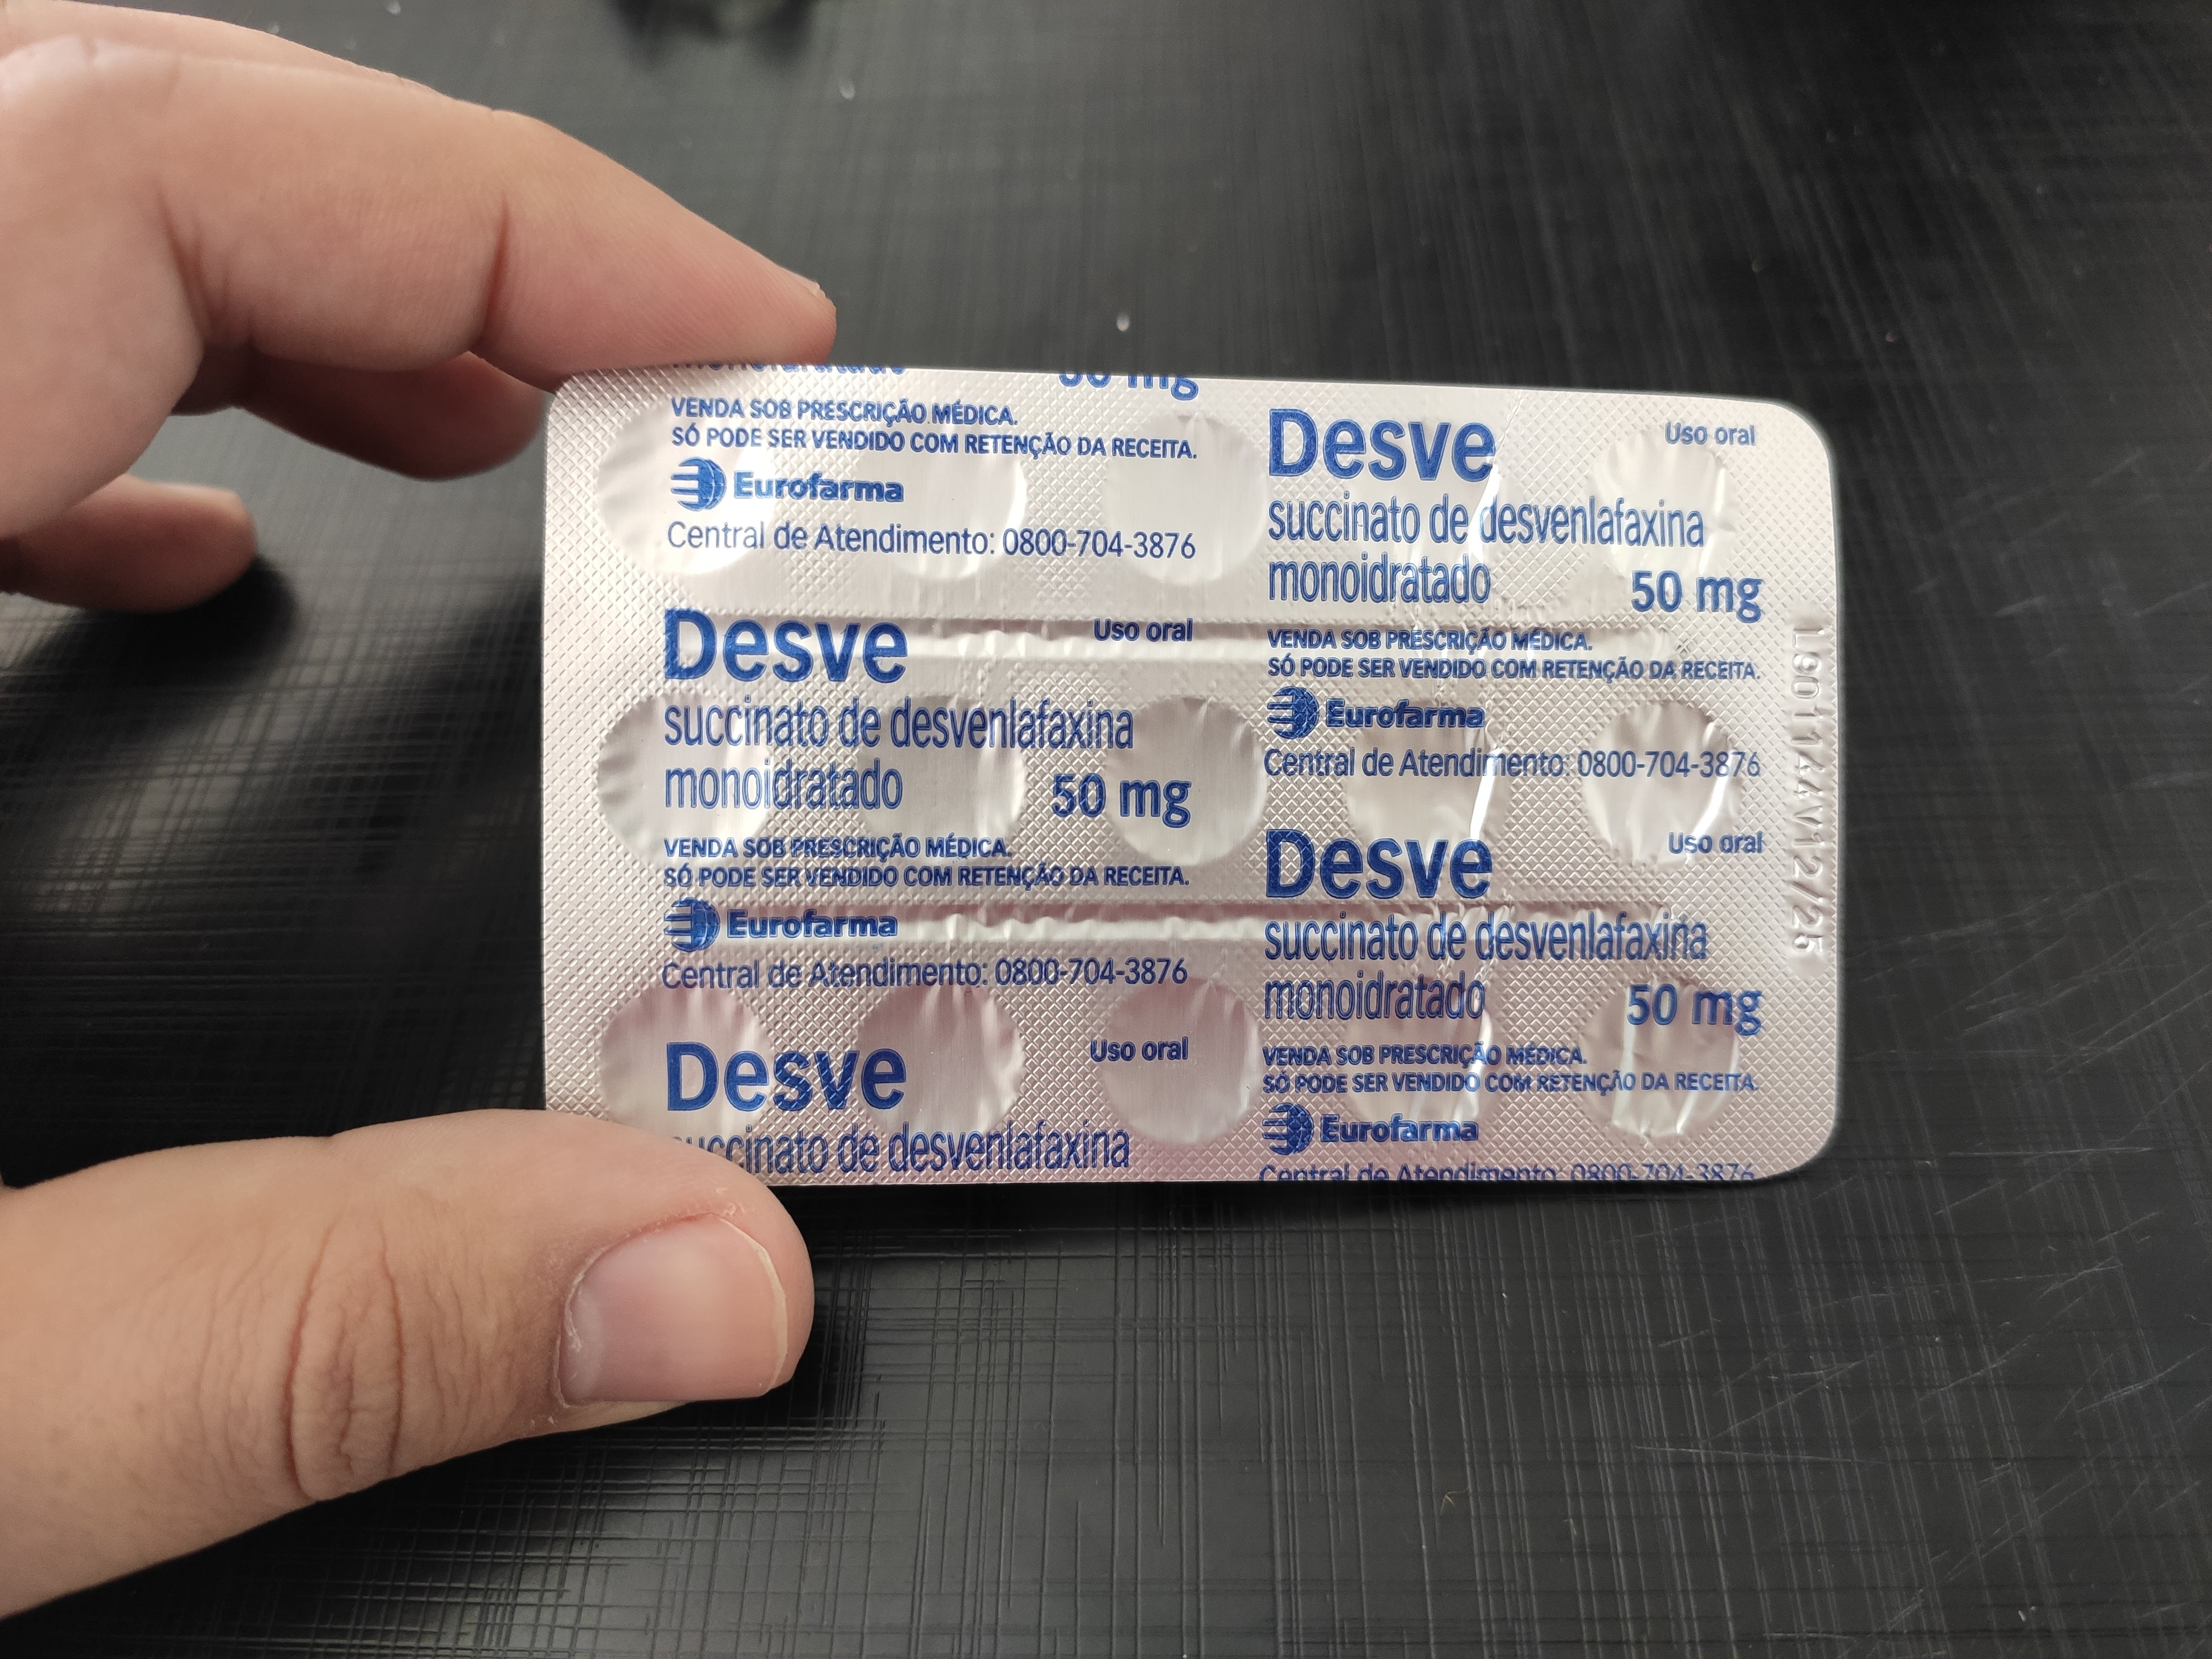
\includegraphics[width=\linewidth]{../pictures/IMG_20240725_110238.jpg}
        \caption*{Fonte: Autor.}
    \end{subfigure}
    \hfill
    \label{fig:fotos:quebint}
\end{figure}

